% This is the Reed College LaTeX thesis template. Most of the work
% for the document class was done by Sam Noble (SN), as well as this
% template. Later comments etc. by Ben Salzberg (BTS). Additional
% restructuring and APA support by Jess Youngberg (JY).
% Your comments and suggestions are more than welcome; please email
% them to cus@reed.edu
%
% See http://web.reed.edu/cis/help/latex.html for help. There are a
% great bunch of help pages there, with notes on
% getting started, bibtex, etc. Go there and read it if you're not
% already familiar with LaTeX.
%
% Any line that starts with a percent symbol is a comment.
% They won't show up in the document, and are useful for notes
% to yourself and explaining commands.
% Commenting also removes a line from the document;
% very handy for troubleshooting problems. -BTS

% As far as I know, this follows the requirements laid out in
% the 2002-2003 Senior Handbook. Ask a librarian to check the
% document before binding. -SN

%%
%% Preamble
%%
% \documentclass{<something>} must begin each LaTeX document
\documentclass[12pt,twoside]{reedthesis}
% Packages are extensions to the basic LaTeX functions. Whatever you
% want to typeset, there is probably a package out there for it.
% Chemistry (chemtex), screenplays, you name it.
% Check out CTAN to see: http://www.ctan.org/
%%
\usepackage{graphicx,latexsym}
\usepackage[french]{babel} 
\usepackage{amsmath}
\usepackage{amssymb,amsthm}
\usepackage[dvipsnames]{xcolor} % tk: for more color
\usepackage{xcolor}
\usepackage{eso-pic}
\usepackage{longtable,booktabs,setspace}
\usepackage{chemarr} %% Useful for one reaction arrow, useless if you're not a chem major
\usepackage[hyphens]{url}
\usepackage{tikz}
\usetikzlibrary{calc}
\newcommand\HRule{\rule{\textwidth}{1pt}}
% Added by CII
\usepackage{hyperref}
\usepackage{lmodern}
\usepackage{float}
\floatplacement{figure}{H}
% End of CII addition
\usepackage{rotating}
\usepackage{upgreek} % tk : pour pouvoir utiliser le symbole µ droit (pas en itallic)
\usepackage{pdfpages}
\usepackage{lscape}
\newcommand{\blandscape}{\begin{landscape}}
\newcommand{\elandscape}{\end{landscape}}
\usepackage[utf8]{inputenc}




% Next line commented out by CII
%%% \usepackage{natbib}
% Comment out the natbib line above and uncomment the following two lines to use the new
% biblatex-chicago style, for Chicago A. Also make some changes at the end where the
% bibliography is included.
%\usepackage{biblatex-chicago}
%\bibliography{thesis}


% Added by CII (Thanks, Hadley!)
% Use ref for internal links
\renewcommand{\hyperref}[2][???]{\autoref{#1}}
\def\chapterautorefname{Chapter}
\def\sectionautorefname{Section}
\def\subsectionautorefname{Subsection}
% End of CII addition

% Added by CII
\usepackage{caption}
\captionsetup{width=5in}
% End of CII addition

% \usepackage{times} % other fonts are available like times, bookman, charter, palatino


% To pass between YAML and LaTeX the dollar signs are added by CII
\title{THÈSE}
\author{Thomas Karaouzene}
\labo{}
% The month and year that you submit your FINAL draft TO THE LIBRARY (May or December)
\date{07 novembre 2017}
\division{}
\advisor{Pierre Ray}
%If you have two advisors for some reason, you can use the following
% Uncommented out by CII
\altadvisor{Nicolas Thierry-Mieg}
% End of CII addition

%%% Remember to use the correct department!
\department{Ingénierie de la Santé, de la Cognition et Environnement (EDISCE)}
% if you're writing a thesis in an interdisciplinary major,
% uncomment the line below and change the text as appropriate.
% check the Senior Handbook if unsure.
%\thedivisionof{The Established Interdisciplinary Committee for}
% if you want the approval page to say "Approved for the Committee",
% uncomment the next line
%\approvedforthe{Committee}

% Added by CII
%%% Copied from knitr
%% maxwidth is the original width if it's less than linewidth
%% otherwise use linewidth (to make sure the graphics do not exceed the margin)
\makeatletter
\def\maxwidth{ %
  \ifdim\Gin@nat@width>\linewidth
    \linewidth
  \else
    \Gin@nat@width
  \fi
}
\makeatother

\renewcommand{\contentsname}{Table of Contents}
% End of CII addition

\setlength{\parskip}{0pt}

% Added by CII
  %\setlength{\parskip}{\baselineskip}
  \usepackage[parfill]{parskip}

\providecommand{\tightlist}{%
  \setlength{\itemsep}{0pt}\setlength{\parskip}{0pt}}

\Acknowledgements{

}

\Dedication{

}

\Preface{

}

\Abstract{

}

	\usepackage{tikz}
% End of CII addition
%%
%% End Preamble
%%
%

\begin{document}

% Everything below added by CII
      \maketitle
  
  \frontmatter % this stuff will be roman-numbered
  \pagestyle{empty} % this removes page numbers from the frontmatter

  
  
      \hypersetup{linkcolor=black}
    \setcounter{tocdepth}{3}
    \tableofcontents
  
      \listoftables
  
      \listoffigures
  
  
  
  \mainmatter % here the regular arabic numbering starts
  \pagestyle{fancyplain} % turns page numbering back on

  \chapter{Investigation génétique et physiologique de la
  globozoospermie}\label{globo}
  
  \section{Introduction sur la
  globozoospermie}\label{introduction-sur-la-globozoospermie}
  
  Comme expliqué précédemment, La globozoospermie est un phénotype rare
  (\textless{} 0.1\% des patients infertiles) mais néanmoins sévère
  {[}\protect\hyperlink{ref-Sen2009}{1}{]} de teratozoospermie menant à
  l'infertilité masculine. Cette anomalie est caractérisée par la présence
  de spermatozoïdes présentant une tête ronde dépourvue d'acrosome et
  d'une pièce intermédiaire désorganisée dans l'éjaculat
  {[}\protect\hyperlink{ref-Singh}{2},
  \protect\hyperlink{ref-Pedersen1974}{3}{]} (\textbf{Figure :
  }\ref{fig:globospz}). En plus des anomalies morphologiques, les
  spermatozoïdes globozoocéphales présentent également des
  désorganisations au niveau moléculaire. Par exemple, le facteur
  spermatique PLC\(\zeta\) requit pour l'activation ovocitaire, est absent
  ou en quantité infime dans les spermatozoïdes globozoocéphales
  {[}\protect\hyperlink{ref-Heytens2009}{4}--\protect\hyperlink{ref-Yoon2008}{6}{]}
  compromettant ainsi l'activation ovocytaire et expliquant le faible taux
  de fécondation observés en IVF (\emph{in vitro} fertilization) et en
  ICSI (intra cytoplasmic sperm injection)
  {[}\protect\hyperlink{ref-Dam2006}{7}{]}. On distingue la
  globozoospermie totale avec 100\% des spermatozoïdes présentant le
  phénotype ou partielle en fonction du taux de spermatozoïdes atteints.
  Bien que l'infertilité masculine soit souvent la résultante de plusieurs
  facteurs, les premières études présentant des patients atteints par un
  phénotype complet {[}\protect\hyperlink{ref-Sen2009}{1}{]} suggéraient
  que la globozoospermie était une exception. De plus les caractéristiques
  morphologiques très typiques des spermatozoïdes laissaient penser à une
  cause monogénique. En 2007, une étude portant sur une famille juive
  ashkénaze comprenant six frères dont trois atteins a pu lier ce
  phénotype à une mutation homozygotes sur le gène \emph{SPATA16} présente
  chez les trois frères atteint {[}\protect\hyperlink{ref-Dam2007}{8}{]}.
  Cependant, dans la même étude, 29 autres patients présentant le même
  phénotype ont été analysés, et pour ceux-ci, aucun variant du gène
  \emph{SPATA16} n'a pu être lié au phénotype
  {[}\protect\hyperlink{ref-Dam2007}{8}{]} indiquant clairement que les
  mutations de ce gène n'étaient pas les seules responsables. En 2011, une
  autre étude portant sur une cohorte de 20 patients Tunisiens a pu mettre
  en évidence une délétion homozygote de 200kb emportant la totalité du
  gène \emph{DPY19L2} chez 15 des 20 patients analysés
  {[}\protect\hyperlink{ref-Harbuz2011}{9}{]}. Les études effectuées
  ultérieurement sur ce phénotype ont ensuite pu montrer que les
  altérations du gène \emph{DPY19L2}, et notamment cette délétion, étaient
  responsables de la majorité des cas de globozoospermie
  {[}\protect\hyperlink{ref-Ray2011}{10},
  \protect\hyperlink{ref-ElInati2012}{11}{]}.
  
  \begin{figure}
  
  {\centering 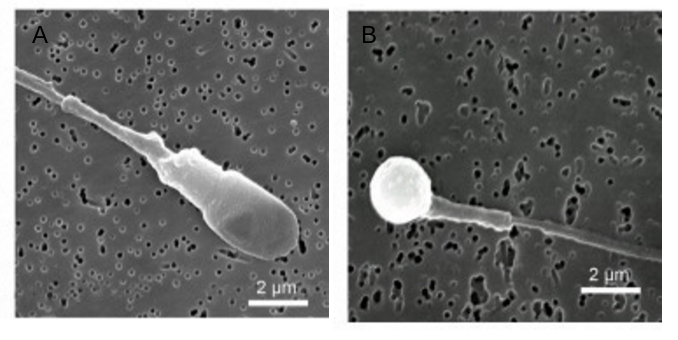
\includegraphics[scale=0.50]{figure/globo_normal_spz} 
  
  }
  
  \caption[Observation au microscope à balayage d'un spermatozoïde normal (**A**) et d'un spermatozoïde globozoocéphale (**B**) (changer les photos avec celles sur lesquelles on voit l'acrosome colorés)]{Observation au microscope à balayage d'un spermatozoïde normal (**A**) et d'un spermatozoïde globozoocéphale (**B**) (changer les photos avec celles sur lesquelles on voit l'acrosome colorés) adapté d'après [@Harbuz2011]}\label{fig:globospz}
  \end{figure}
  
  En 2012, le développement d'un modèle murin KO \emph{Dpy19l2}\(^{-/-}\)
  a permis de mieux comprendre les mécanismes moléculaires impliqués dans
  la globozoospermie causée par la délétion du gène \emph{DPY19L2} chez
  l'humain {[}\protect\hyperlink{ref-Pierre2012}{12}{]}. Ce modèle de
  souris KO présentant les mêmes caractéristiques que les patients humains
  ; Tout d'abord, ces souris étaient infertiles et présentaient des
  spermatozoïdes globozoocéphales (\textbf{Figure : }\ref{fig:mouseglobo})
  mais aussi et surtout, l'ensembles des autres dysfonctionnements étaient
  retrouvés, c'est à dire : l'absence de l'acrosome, les défauts
  morphologiques du noyau, de l'enveloppe nucléaire et de l'acroplaxome
  ainsi que le mauvais positionnement de la manchette
  {[}\protect\hyperlink{ref-Pierre2012}{12}{]}. Ainsi il a pu être
  démontré que la protéine Dpy19l2 étaient principalement exprimée dans le
  spermatide et plus spécifiquement dans la membrane nucléaire interne
  faisant face à la vésicule acrosomale et que l'absence de cette protéine
  entrainait la déstabilisation à la fois de la lamine nucléaire, de la
  jonction entre l'acroplaxome et l'enveloppe nucléaire
  {[}\protect\hyperlink{ref-Pierre2012}{12}{]}.
  
  \begin{figure}
  
  {\centering 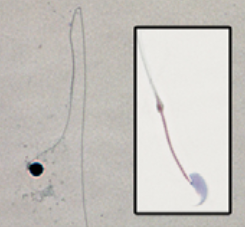
\includegraphics[scale=0.8]{figure/mouse_globo_spz} 
  
  }
  
  \caption[Comparaison entre les spermatozoïdes des souris *Dpy19l2*$^{-/-}$ (à gauche) et les souris sauvages *Dpy19l2*$^{+/+}$ (à droite)]{Comparaison entre les spermatozoïdes des souris *Dpy19l2*$^{-/-}$ (à gauche) et les souris sauvages *Dpy19l2*$^{+/+}$ (à droite) d'après [@Pierre2012]}\label{fig:mouseglobo}
  \end{figure}
  
  \newpage
  
  \section{\texorpdfstring{Résultats 1 : Les mécanismes mutationnels
  entrainant la délétion au locus de \emph{DPY19L2} chez
  l'humain}{Résultats 1 : Les mécanismes mutationnels entrainant la délétion au locus de DPY19L2 chez l'humain}}\label{mecamut}
  
  \subsection{Article n° 1:}\label{article-n-1}
  
  \textbf{Fine Characterisation of a Recombination Hotspot at the
  \emph{DPY19L2} Locus and Resolution of the Paradoxical Excess of
  Duplications over Deletions in the General Population}
  
  Coutton C, Abada F, \textbf{Karaouzène T}, Sanlaville D, Satre V,
  LunardiJ, Jouk PS, Arnoult C, Thierry-Mieg N, Ray PF
  
  \textsuperscript{*} Co-premiers auteurs
  
  PLOS GeneticS, Mars 2013
  
  \newpage
  
  \subsubsection{Contexte et objectifs}\label{contexte-et-objectifs}
  
  Chez les mammifères il existe trois paralogues de \emph{DPY19L2} de
  fonctions encore inconnues et un pseudogène présentant une très forte
  homologie de séquence (\textgreater{} 95\%)
  {[}\protect\hyperlink{ref-Carson2006}{13}{]}. Chez l'Homme, ce gène est
  flanqué de deux séquences présentant une forte homologie
  (\textgreater{}95\%) d'une taille de 28kb. Ces séquences appelées LCRs
  (\emph{low copy repeats}) représentent une large portion du génome
  humain {[}\protect\hyperlink{ref-Cheung2003}{14},
  \protect\hyperlink{ref-Bailey2002}{15}{]} et vont, de par leur homologie
  favoriser les duplications de gènes jouant ainsi un rôle important dans
  l'évolution des génomes des vertébrés
  {[}\protect\hyperlink{ref-Walsh2003}{16},
  \protect\hyperlink{ref-Ohno1970}{17}{]}. Dans le cas de \emph{DPY19L2},
  ces LCRs vont, au cours de la méiose entrainer la venue de
  recombinaisons homologues non-allélique (NAHR) donnant lieu soit à une
  délétion du gène \emph{DPY19L2} et la formation d'un ADN circulaire
  comprenant le gène soit à un allèle possédant deux copies du gène tandis
  que l'autre n'en possède aucune
  {[}\protect\hyperlink{ref-Harbuz2011a}{18}{]}.
  
  Ce mécanisme de NAHR devrait, en théorie, engendrer la formation de plus
  d'allèles délétés que d'allèles dupliqués puisque les cas présentés en
  figures \ref{fig:nahr} - \textbf{2} et \ref{fig:nahr} - \textbf{3}
  induisent la formation d'un allèle délété tandis que seul le cas
  \ref{fig:nahr} - \textbf{3} forme un allèle dupliqué
  {[}\protect\hyperlink{ref-Liu2012}{19}{]}. Cependant, les données mises
  à disposition par la base de données
  \href{http://dgv.tcag.ca/dgv/app/home}{\emph{Database of Genomic
  Variants}} (DGV) {[}\protect\hyperlink{ref-MacDonald2014}{20}{]}
  indiquent un excès de duplication puisque sur un total de 6575 individus
  analysés, 83 duplications et de 26 délétions hétérozygotes ont été
  observées pour le locus de \emph{DPY19L2}.
  
  Ainsi, dans cette étude, notre équipe a cherchée à caractériser
  précisément le mécanisme génétique et les facteurs favorisant la
  survenue par NAHR de la délétion homozygote récurrente emportant
  totalement le gène DPY19L2. De même, nous avons tenté de résoudre le
  paradoxe observé entre le modèle théorique de NAHR et la fréquence des
  allèles observée dans la population générale afin de confirmer les
  données fournies dans les bases de données et ainsi écarter l'hypothèse
  d'un biais causé par la présence du pseudogène \emph{DPY19L2P1} très
  homologue avec \emph{DPY19L2}
  {[}\protect\hyperlink{ref-Carson2006}{13}{]}.
  
  Dans ce contexte j'ai pu participer à divers manipulations de biologie
  moléculaire tel que l'extraction d'ADN spermatique, quantification des
  délétions / duplications \emph{de novo}. De même, j'ai pu contribuer au
  divers analyses statistiques.
  
  \newpage 
  
  \begin{figure}
  
  {\centering \includegraphics[scale=0.5]{figure/nahr_process} 
  
  }
  
  \caption[Représentation schématique du mécanisme de NAHR]{Représentation schématique du mécanisme de NAHR adapté d'après [@Liu2012] : Lors d'un NAHR interchromatidien, un allèle dupliqué et un allèle délété sont formés. Lors d'un NAHR intrachrmatidien, seule un allèle délété est produit, en même temps qu'un petit ADN circulaire qui sera éliminé par la suite.}\label{fig:nahr}
  \end{figure}
  
  \newpage
  
  \includepdf[pages=-]{bib/DPY19L2_2013}
  
  \newpage
  
  \subsubsection{Principaux résultats}\label{principaux-resultats}
  
  Alors que les résultats précédents confirment un excès de l'allèle
  dupliqué de \emph{DPY19L2} dans la population générale, nous avons par
  la suite cherché à déterminer les fréquences de duplications / délétions
  \emph{de novo} de ce même locus. Ceci ayant pour but de déterminer si
  cet exces est dû à une séléction de l'allèle dupliqué ou au fait que
  celui-ci était effectivement produit plus fréquement que l'allèle
  délété. Pour ce faire nous avons quantifié le taux d'apparition de ces
  événements génétiques à partir d'ADN spermatique. Les spermatozoïdes
  étant le produits direct de la méiose, ils sont donc les reflets
  d'haplotypes produits \emph{de novo}. Pour cela, nous avons analysé par
  PCR digitale l'ADN spermatique de trois donneurs ainsi que l'ADN
  spermatique constitué d'un mix provenant de ces trois donneurs. Leur ADN
  a tout d'abor été dilué en série de sorte à ce qu'environ 25\% des 96
  puits de la PCR contiennent un événement (délétion ou duplication).
  Ainsi, en acceptant qu'un génome haploïde humain représente 3pg, 50ng
  d'ADN spermatique furent déposés dans chaque puit pour la PCR spécifique
  à la délétion, et 100ng dans chaque puit spécifiques à a duplication.
  Chaque puit contient donc une partie de cette charge d'ADN initiale. La
  distribution de cette charge d'ADN au sein des 96 puits peut donc
  s'apparier à un tirage sans remise, la probabilité qu'un puit soit
  positif pour un événement chromosomique (duplication ou délétion) peut
  donc être modélisé par une loi hypergéométrique (\textbf{Équation} :
  \eqref{eq:hypergeo}). Nous permettant ainsi d'estimer la fréquence
  duplication / délétion \(\lambda\) pour chaque donneur
  (\textbf{Équation} : \eqref{eq:lambda}).\\
  
  \begin{equation} 
  \frac{\frac{(N - R)!}{W!(N-R-W)!}}{\frac{N!}{W!(N-W)!}} = \frac{(N-R)!(N-W)!}{N!(N-W-R)!} = \prod_{i=0}^{R-1}{\frac{N-W-i}{N-i}}
  \label{eq:hypergeo}
  \end{equation}
  
  \begin{equation} 
  \lambda = \frac{R}{N}
  \label{eq:lambda}
  \end{equation}
  
  Où :\\
  . \(N\) : représente le nombre de copie de chromosome 12 dans la charge
  d'ADN initiale (1.6x10\({^6}\) pour la PCR spécifique à la délétion,
  3.2x10\({^6}\) pour la PCR spécifique à la duplication)\\
  . \(W = \frac{N}{96}\) correspond au nombre de copiede chromosome 12 par
  puit\\
  . \(R\) représente le nombre total de recombinaison observées
  
  L'interval de confiance (IC) à 95\% est ensuite calculé grâce à une loi
  binomiale de sorte à modéliser la dilution initiale pour obtenir l'ADN
  d'\emph{entrée}. Le puit contenant le \emph{pool} des trois ADN
  spermatique est donc celui ayant les résultats les plus robustes, l'IC
  étant le plus resséré, et permet donc d'établir le taux de délétion
  \emph{de novo} à 1.8 x 10\(^{-5}\) (IC 95\% : 1.4x 10\(^{-6}\); 2.2x
  10\(^{-6}\)) tandis que le taux de duplication \emph{de novo} est estimé
  à 7.7 x 10\(^{-6}\) (IC 95\% : 6.1 x 10\(^{-6}\); 9.7 x 10\(^{-6}\))
  montrant un enrichisement environ deux fois supperieur des délétion par
  rapport aux duplications sur le site de \emph{DPY19L2}.
  
  Ainsi, de manière paradoxale, les délétion \emph{de novo}
  apparaitraient, au cours de la méïose, deux fois plus fréquement que les
  dupliquation \emph{de novo} tandis que l'allèle dupliqué est trois fois
  plus fréquent que l'allèle délété dans la population générale. Cet effet
  pourrait en partie être due aux effets de séléction naturelle. En effet,
  Bien qu'à notre connaissance, les femmes portant l'allèle délété à
  l'état homozygote ne soient caractérisées par aucun phénotype, les
  hommes, eux sont 100\% infertiles tandis que l'allèle dupliqué ne
  subirait aucune séléction.
  
  Cette étude a également été pour notre équipe l'occasion d'effectuer une
  étude plus approfondie des LCRs flanquant le locus de \emph{DPY19L2}.
  Pour cela, nous avons génotypé 20 SNPs spécifiques des LCRs télomériques
  et centromériques. À partir de ces données, 5 points de cassures
  distincts (BP1-5) ont pu être identifiés sur les 185 allèles recombinés
  étudiés (108 délétés et 77 dupliqués). L'ensemble de ces points de
  cassures sont localisés dans une région d'environ 1150 pb. L'analyse
  bioinformatique de cette région a permi de mettre en évidence, au centre
  de cette région, 13 nucléotides (CCNCCNTNNCCNC) constituant un site de
  reconnaissance consensus de la protéine PRDM9. Cette protéine à doigts
  de zinc étant connue pour son rôle central dans l'activation de la
  transcription dans les premères phases de la prophase méiotique ainsi
  que pour être à impliqué dans les mécanismes de recombinaisons
  chromosomique au cours de la méiose chez l'humain et la souris
  {[}\protect\hyperlink{ref-Parvanov2010}{21},
  \protect\hyperlink{ref-Baudat2010}{22}{]}.
  
  \newpage
  
  \section{Résultat 2 : La transcriptomique}\label{transcriptome}
  
  \subsection{Article n° 2:}\label{article-n-2}
  
  \textbf{Comparative testicular transcriptome of wild type and
  globozoospermic Dpy19l2 knock out mice}
  
  \textbf{Karaouzène T} , El Atifi M, Issartel JP, Grepillat M, Charles
  Coutton C, Martinez D, Arnoult C and Ray PF
  
  Basic and Clinical Andrology, 2013
  
  \newpage
  
  \subsubsection{Contexte et objectifs}\label{contexte-et-objectifs-1}
  
  Dans des études précédentes, notre équipe à réussit à démontrer que la
  protéine DPY19L2 était localisée dans la membrane interne des noyaux des
  spermatides pendant la spermatogénèse et qu'elle était nécessaire pour
  fixer l'acrosome au noyau {[}TODO: insert ref{]}. De même, nous avons pu
  mettre en évidence que dans des cellules HEK cette protéine colocalisait
  avec la protéine SUN5 et que \emph{Dpy19l2} pourrait être un partenaire
  de SUN5{[}\protect\hyperlink{ref-Pierre2012}{12}{]}. Nous avons cherché
  à observer si, comme la protéine SUN5. Chez la souris, la protéine Sun1
  est elle aussi nécéssaire à la gamétogénèse et est connue pour permettre
  l'intéraction entre le noyau et les télomères
  {[}\protect\hyperlink{ref-Ding2007}{23}{]}. Dans cette étude nous avons
  donc chercher à savoir si l'absence de la protéine Dpy19l2 pouvait
  entrainer des dérèglement transcriptionelle qui pourrait, entre autre,
  expliquer l'absence de la protéine PLC\(\zeta\) dans les spermatozoïdes
  globozoocéphales.\\
  De plus, au cours de l'elevage des souris \emph{Dpy19l2} KO au sein de
  notre laboratoir nous avons pu observé un excès de naissance de souris
  mâle lorsque l'on croisait deux souris \emph{Dpy19l}\(^{+/-}\). Ainsi,
  en comparant les sexes des souris obtenues lors de 6 premières
  naissances (\emph{Birth 1-6}) on observe un total de 28 souris mâles
  pour 16 souris femelles. La p-valeur obtenue en effectuant un test de
  \(\chi^2\) comparant ces deux effectifs était égale à 0.0486272 laissant
  supposé l'existence d'un réel, bien que faible, enrichissement en souris
  mâles.
  
  C'est donc afin d'expliquer l'abscence de la protéine
  \emph{Plc}\(\zeta\) dans les spermatozoïdes des souris
  \emph{Dpy19l2}\(^{-/-}\) ainsi que l'enrichissement en souris mâle dans
  les naissances issues d'accouplement de souris \emph{Dpy19l2}\(^{+/-}\)
  que nous avons effectué une analyse comparative du transcriptome
  testiculaire de deux souris \emph{Dpy19l2}\(^{+/+}\)
  (S1\textsuperscript{+} et S2\textsuperscript{+}) et deux souris
  \emph{Dpy19l2}\(^{-/-}\) (S1\textsuperscript{-} et
  S2\textsuperscript{-}) ayant pour but de mettre en évidence d'eventuels
  dereglement transcriptionels chez la souris KO.
  
  Dans cette étude j'ai pu effectuer l'intégralité des manipulation de
  biomoléculaire tel que la mise en place du protocole de génotypage des
  souris, l'extraction de l'ARN testiculaire de souris et l'analyse sur
  puce, ainsi que l'intégralité de l'analyse bioinformatique des
  résultats.
  
  \newpage
  
  \begin{figure}
  
  {\centering \includegraphics{thesis_files/figure-latex/plotborn-1} 
  
  }
  
  \caption[Quantification des sexes des souris observées lors de chaque naissances issues d'un croisement de deux souris hétérozygotes *Dpy19l2* +/-]{Quantification des sexes des souris observées lors de chaque naissances issues d'un croisement de deux souris hétérozygotes *Dpy19l2* +/-}\label{fig:plotborn}
  \end{figure}
  
  \newpage
  
  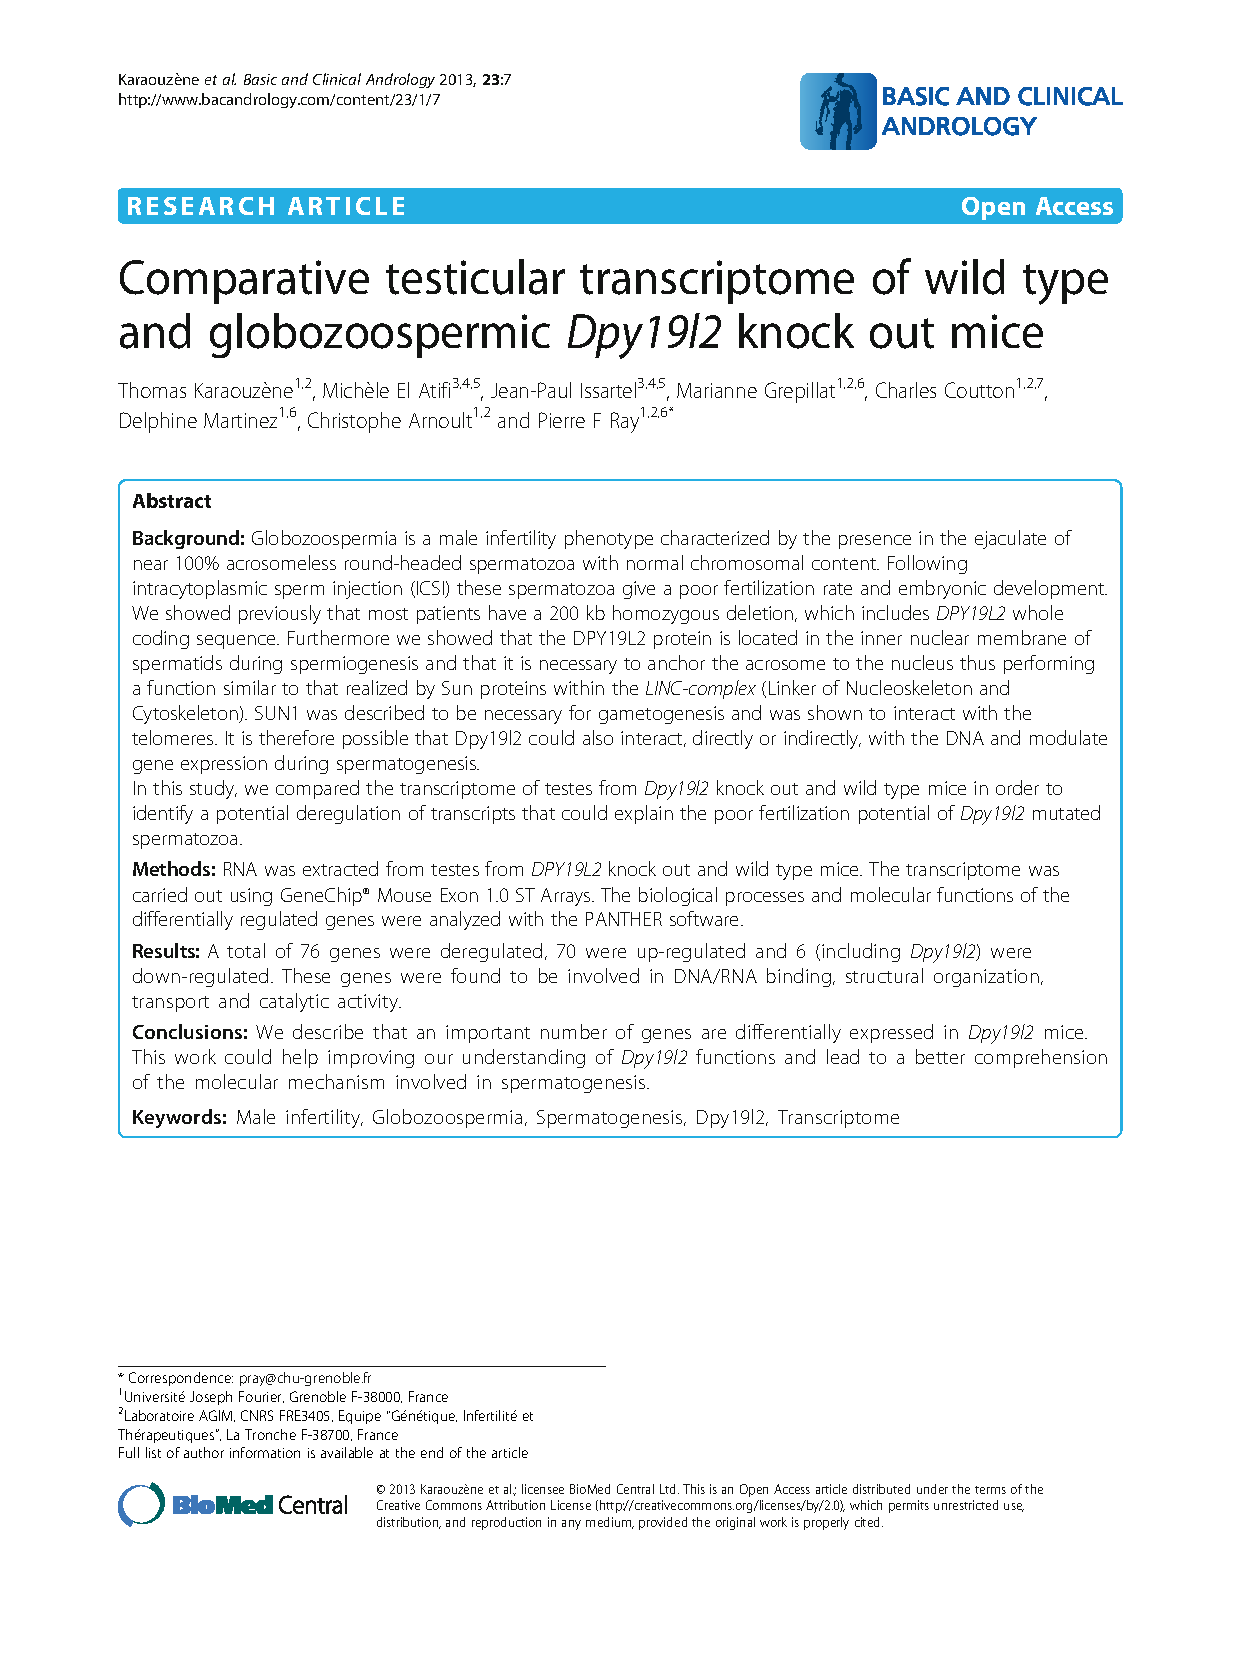
\includepdf[pages=-]{bib/12610_2013_Article_8.pdf}
  
  \newpage
  
  \subsubsection{Principaux résultats :}\label{principaux-resultats-1}
  
  Pour effectuer ces analyses, nous avons donc extrait l'ARN testiculaire
  des 4 souris que nous avons ensuite hybridé sur des puces à ADN
  Affymetrix GeneChip® Mouse Exon 1.0 contenant des sondes pour 35.557
  gènes murins. Cette étape nous a alors permi d'obtenir pour chacune des
  4 souris les valeurs d'expression testiculaire de l'ensemble de leurs
  gènes. Pour chacun de ces gènes, nous avons donc chercher à savoir s'ils
  étaient différentiellement exprimés chez les sours S1\textsuperscript{-}
  et S2\textsuperscript{-} lorsqu'on comparait leur expression avec celle
  des souris S1\textsuperscript{+} et S2\textsuperscript{+}. Pour cela,
  nous avons calculé quatre ratios (R1, R2, R3 et R4) (\textbf{Équation} :
  \eqref{eq:micerate}). Les gènes pour lesquels au moins 3 de leurs ratio
  étaient \(\ge\) 1,7 furent considérés comme sur-exprimés tandis que ceux
  pour lesquels 3 de leurs ratio étaient \(\le\) 0,58 (\(\frac{1}{1,7}\))
  furent considérés comme sous-exprimés.\\
  
  \begin{equation} 
  \begin{split}
  \forall gene \in & \ \{genes\ in\ array\}: \\
  \\
  & R1_{gene} = \frac{exp_{gene}(S1^-)}{exp_{gene}(S1^+)} \ \ \ \ R2_{gene} = \frac{exp_{gene}(S2^-)}{exp_{gene}(S1^+)} \\
  & R3_{gene} = \frac{exp_{gene}(S1^-)}{exp_{gene}(S2^+)} \ \ \ \ R4_{gene} = \frac{exp_{gene}(S2^-)}{exp_{gene}(S2^+)} 
  \label{eq:micerate}
  \end{split}
  \end{equation}
  
  De cette manière cette étude a pu mettre en évidence la sous-expression
  de 6 gènes (incluant \emph{Dpy19l2}) et la sur-expression de 70 gènes
  chez les souris \emph{Dpy19l2}\(^{-/-}\). Parmi ces gènes, nous ne
  figurait pas \emph{Plc}\(\zeta\) indiquant que l'absence de cette
  protéine chez les spermatozoïdes globozoocéphales n'étaient pas
  directement dûe à un dysfonctionnement transcriptionel. Afin de prédire
  les fonction moléculaire dans lesquels étaient impliqués ces gènes, nous
  nous sommes servi du logiciel PANTHER
  {[}\protect\hyperlink{ref-Mi2017}{24}{]}. Ainsi, nous avons pu constater
  que 23 gènes codant pour des protéines de liaison étaient dérégulés
  (\textbf{Figure : }\ref{fig:plotmolfunction} - \textbf{A}), dont sont
  des protéines de liaison aux acides nucléiques (\textbf{Figure :
  }\ref{fig:plotmolfunction} - \textbf{B}) suggérant que \emph{Dpy19l2}
  pourrait effectivement intéragir avec l'ADN. D'autre fonctions
  moléculaires telles que l'activité catalytique, la régulation de la
  transcription et des protéines ayant des fonctions structurelles étaient
  égallement dérégulées chez les souris KO. Ces derniers sont
  particulièrement intéréssant lorsque l'on sait que les spermatozoïdes
  globozoocéphales sont caractérisés par plusieurs défauts structurels.
  
  Cette étude a pour nous été l'occasion de mieux caractériser la protéine
  \emph{Dpy19l2} chez la souris. Nous avons ainsi pu montrer que les
  souris \emph{Dpy19l2}\(^{-/-}\) présentaient des déréglements
  transcriptionels affectant plusieurs fonctions moléculaires pouvant
  ainsi expliquer, du moins en partie, les nombreux défauts morphologiques
  caractérisant les spermatozoïdes globozoocéphales. De même, nous avons
  pu observer un déréglement de nombreux gènes impliqués dans la liaison
  d'acide nucléique et de protéine pouvant ainsi expliquer les défauts
  d'ancrage de l'acrosome au noyau chez les spermatozoïdes
  globozoocéphales.
  
  Ces résultats ne nous ont cependant pas permis d'expliquer l'abscence de
  la protéine Plc\(\zeta\) dans le spermatozoïde globocéphale murin
  l'expression du gène \emph{Plc}\(\zeta\) n'ayant montré aucune
  dérugulation chez la souris \emph{Dpy19l2}\textsuperscript{-/-}. De
  même, aucun des gènes retrouvés comme dérégulé ne nous a permis
  d'expliquer le biais de sexe que nous avions observés. Cela n'a pas été
  une surprise pour nous puisque après avoir entamé notre étude, une
  dernière portée issues d'un croisement de souris
  \emph{Dpy19l2}\textsuperscript{+/-} a vus le jours. Celle-ci état
  composée de 4 souriceaux mâles et de 4 souriceaux femelles. Ainsi, avec
  un total de 32 souris mâles pour 20 souris femelles, la p-valeur de
  notre test du \(\chi^2\) à 0.0635765 laissant cete fois-ci supposer la
  non-existence d'un biais de sexe dans les naissances issues d'un
  croisement de souris \emph{Dpy19l2}\textsuperscript{-/-}.
  
  \newpage 
  
  \begin{figure}
  
  {\centering \includegraphics{thesis_files/figure-latex/plotmolfunction-1} 
  
  }
  
  \caption[Principales fonctions moléculaires affectées chez les souris *Dpy19l2* KO]{Principales fonctions moléculaires affectées chez les souris *Dpy19l2* KO  :  **A** : Liste des fonctions moléculaires affectées : Bndn = Binding, Ctly = Catalytic, Trnsc = Transcription, Strm = Structural molecule, Rcpt = Receptor. **B** : Détails des fonctions moléculaires affectées par les gènes dérégulés}\label{fig:plotmolfunction}
  \end{figure}
  
  \chapter*{Conclusion et discussion}\label{conclusion-et-discussion}
  \addcontentsline{toc}{chapter}{Conclusion et discussion}
  
  L'infertilité Est une problématique à laquelle font face entre 10 et
  15\% des couples humains {[}\protect\hyperlink{ref-Boivin2007a}{25}{]}
  faisant de cette pathologie un enjeux de santé publique. Bien que les
  causes de ce phénotypes puissent être multifactorielles et aquises au
  cours de la vie de l'individus, notamment suite à des infections du
  système urogénitale ou encore à des perturbations du système
  endocrinien, la composante génétique est extrêmement importante. À jour,
  malgres les efforts de nombreuses équipes, incluant lma notre, seulement
  une poignée de gène ont pu être relié à ce phénotype. De plus, pour
  nombre d'entre eux, les bases moléculaires reliant une mutation au
  phénotype d'infertilité restent inconnues.
  
  Dès lors, la première partie de mon travail de thèse à consister à
  contribuer à la caractérisation du phénotype de globozoospermie. Ce
  phénotype, entrainant la production dse 100\% de spermatozoïdes à têtes
  rondes et dépourvus d'acrosomes est dans principalement causé, chez
  l'humain, par une délétion homozygote récurrente entrainant la totalité
  de la séquence du gène \emph{DPY19L2}. Ainsi, dans deux études
  différentes, nous avons pu, dans un premiers temps, mieux caractériser
  les mécanismes moléculaires responsables de cette délétion. Ainsi, nous
  avons pu mettre en évidence cinq points de cassures aux niveau des LCRs
  flanquant la séquence de \emph{DPY19L2} chez l'humain. Ceux-ci étant
  tous concentrés dans une région d'environ 1150 pb contenant en son
  centre un site de reconaissance consensus de la protéine PRDM9 connue
  pour son implication dans la recombinaison chromosimique chez l'humain
  et la souris {[}\protect\hyperlink{ref-Parvanov2010}{21},
  \protect\hyperlink{ref-Baudat2010}{22}{]}. Cette même étude a également
  permis de démontrer que les effets de la séléction naturelle étaient
  responsables du paradoxe consistant à observer plus fréquemment, dans la
  population générale, l'allèle dupliqué à ce locus que l'allèle délété
  tandis que \emph{de novo} l'allèle délété est produit, en théorie et en
  pratique, plus fréquement que l'allèle dupliqué. L'étude de ce phénotype
  nous a part la suite poussé à étudié le modèle murin KO
  \emph{Dpy19l2}\textsuperscript{-/-} présentant le même phénotype que
  l'humain. Afin d'expliquer l'absence de la protéine PLC\(\zeta\) chez
  l'humain globozoosperme, nous avecs effectués une analyse comparatives
  des transcriptomes testiculaires de souris sauvages
  \emph{Dpy19l2}\textsuperscript{+/+} et KO
  \emph{Dpy19l2}\textsuperscript{-/-}. Bien qu'aucun déréglement
  transcriptionel n'est pu être observé pour le gène \emph{Plc}\(\zeta\)
  cette étude nous a permis de mettre en évidence un total de 75 gènes
  présentant des dérégulations transcriptionelles pouvant expliquer en
  partie les anomalies physiologiques et morphologiques des spermatozoïdes
  des souris\emph{Dpy19l2}\textsuperscript{-/-}.
  
  Esuite, notre équipe ayant, entre \ldots{} et \ldots{}, a effectué le
  séquençage exomique de plusieurs patients présentant tous un phénotype
  d'infertilité, la seconde partie de mon travail de thèse a été de mettre
  au point un pipeline permettant l'analyse des données générées lors du
  processus de séquençage. Celui-ci ayant pour vocation première de mettre
  en évidence les variants responsables des phénotypes de ces patients.
  Contrairement à la plupart des pipelines d'analyse de données WES
  existant, clui-ci prend en charge l'ensemble des étapes de l'analyse
  allant de l'alignement des \emph{short-reads} sur le génome de référence
  jusqu'à la priorisation des variants en passant bien évidemment par
  l'appel des variants et leur annotation. Les résultats de chacune de ces
  étapes pouvant être controlés et personalisés grâce à des paramètres
  ajustables. L'alignements des \emph{reads} est effectué par le logiciel
  MAGIC tandis que les variants et leur gnotypes sont appelés par un
  algorithme développé dans notre laboratoir spécifiquement conçu pour
  analyser les informations fournies par MAGIC et dont les paramètres sont
  ajustables en fonctions de la distribution des pourcentages de
  \emph{reads} variants observés dans les données analysées. Pour
  l'annotation nous avons utilisé plusieurs ressources exterieures tel que
  le logiciel Variant Effect Predictor qui va nous informer de l'effet
  d'un variant sur l'ensemble des transcrits qu'il chevauche. De même, les
  bases de données ExAC ESP6500 ou encore 1KG nous donne une indication de
  la fréquence des variants dans la population générale. Une fois ces
  étapes effectuées, nous avons mis en place plusieurs filtres succesifs
  afin d'éliminer de nos listes les variants ayant le moins de chances
  d'être responsables du phénotypes des différentes patients. Ceux-ci
  s'appuient à la fois sur les critères qualité des résultats de
  séquençage, le génotype des variants, leur fréquence ou encore leur
  impact sur la protéine.
  
  L'efficacité de ce pipeline a pu être démontré grâce à son utilisation
  utilisation sur des cas familiaux mais aussi sur des cohortes
  d'individus non apparentés. Ainsi, nous avons pu dans un premier temps
  confirmer l'importance de l'implication du gène \emph{DNAH1} dans le
  syndrome MMAF en le retrouvant muté chez \ldots{} de nos patients.
  Ensuite, dans un second temps, ce pipeline nous a permis de mettre en
  évidence un total de 5 nouveaux dans des phénotypes d'infertilité
  masculine et féminine. Ainsi les gènes \emph{CFPA43}, \emph{CFAP44},
  retrouvés respectivement mutés chez \ldots{} et \ldots{} de nos patients
  ont pu être liés à leur syndrome MMAF. Aussi, une même mutation
  impactant le gène PATL2 a pu être relié au phénotype de déficience
  méiotique ovocytaire de cinq femmes. Pour finir, des mutations sur les
  gènes \emph{SPINK2} et \emph{PLC}\(\zeta\), ont elles aussi pu être
  liées aux phénotypes d'azoospermie et d'echec de fécondation dont
  étaient atteins deux fratries.
  
  Ces résultats sont cependant à relativiser puisque pour plusieurs de nos
  patients, aucun candidat n'a pu être identifié. Plusieurs raison peuvent
  expliquer cela. Tout d'abord, au cours des analyses décrites dans ces
  manuscrits nous nous concentrons uniquements sur les SNPs et les indels.
  Cependant de nombreux logiciels tel que \ldots{}, \ldots{} ou encore
  \ldots{} permettent de détecter des CNVs à partir de données WES et / ou
  WGS. Les stratégies de prédictions de ces logiciels pouvant être
  êxtremement différents, le profil des CNVs détécté ou non le sera aussi
  {[}ref {]}. Ainsi, dans des analyses non décrites ici, j'ai pu chercher
  à identifier des CNVs à partir de nos données d'exome à l'aide du
  logiciel ExomeDepth {[}REF{]}. Cette approche a été extrêmement
  concluante puisqu'elle a permi d'identifier une délétion homozygote sur
  le gène \emph{WDR66} de \ldots{} de nos patiens pour lesquels aucun
  candidat n'avait été alors identifié. Ces délétions ont ensuite pu être
  confirmées par PCR et la caractérisation de ce gène est actuellement en
  cours au sein de notre équipe. Au vu de cette réussite, il est désormai
  prévu d'intégrer ce genre d'analyse de manière automatique et
  systématique au sein de notre pipeline. Pour les autres patients n'ayant
  eu aucun candidat identifié, il est possible que le choix de la
  stratégie d'un séquençage exomique plutôt que du génome entier ait
  masqué la cause génétique du phénotype de certains de nos patients. En
  effet, dans ces analyses, nous nous sommes concentrés sur l'analyse des
  variants situés dans les parties codantes \textbf{uniquement}. Ainsi les
  variants situés par exemple dans les microARN n'ont pu être observés.
  Or, les microARN jouent un rôle important dans la régulation génique
  principalement en influant sur la stabilité d'ARNm cibles et sont
  présent en grande quantité au sein des cellules germinales et leur
  importance dans la spermatogénèse a déjà été démontrée chez la souris
  {[}\protect\hyperlink{ref-Comazzetto2014}{26}{]} ainsi que plus
  récemment chez d'autres mammifères dont l'Humain
  {[}\protect\hyperlink{ref-Chen2017}{27}{]} laissant penser que des
  defauts altérants ces microARN pourraient entrainer des
  dysfonctionnement de la spermatogenèse. Aussi, il faut noter que les
  analyses WES \textbf{et} WGS ne permettent pas d'observer les défauts
  épigénétiques, or, ceux-ci représentent une part croissante des causes
  impliquées dans les cas d'infertilité masculine
  {[}\protect\hyperlink{ref-Carrell2011}{28}{]}. Aussi, au vus du grand
  nombre de gène impliqué dans la spermatogénèse il est très possible que
  les causes génétique responsables d'un même phénotype puissent être très
  hétérogène. Par exemple, dans le cas de l'analyse de la cohorte de
  patients MMAF, \ldots{} variants subsistaient après avoir appliquer
  l'ensemble des filtres. Ces variants impactaient \ldots{} gènes
  différents parmi lesquels \ldots{} étaient retrouvé muté chez uniquement
  un seul des \ldots{} patients de la cohorte. Au vu de se nombre
  important de gène, il est très compliqué d'effectué des analyses
  poussées sur l'ensemble d'entre eux. Dès lors, il est possible que la
  cause génétique responsable du phénotype d'un patient soit ``noyé''
  parmi les nombreux variants restant mettant ainsi en évidence la
  nécéssité de créer de nouveaux filtres afin de pouvoir réduire encore
  cette liste.
  
  C'est dans ce but que notre équipe travail actuellement au développement
  du score MutaScript. Ce score a pour but de classer l'ensemble des
  transcrit codant en fonction de leur charge mutationnelle avec l'idée
  sous-jacente que les transcrits les plus mutés dans la population
  générale ne sont probablement pas impliqués dans des pathologies sévères
  à transmission Mendélienne, \emph{a contrario} ceux retrouvés comme
  n'étant pas / peu mutés le sont probablement. Pour ce faire, le score
  MutaScript repose sur trois (\ldots{}). La première étant le jeu de
  transcrit fournit par Ensembl
  {[}\protect\hyperlink{ref-Aken2017}{31}{]}. Afin de connaitre la charge
  mutationnelle de ces transcrits, nous nous sommes basées sur les
  variants mis à disposition par ExAC
  {[}\protect\hyperlink{ref-Lek2016}{32}{]} qui réunit les données d'exome
  de 60.706 individus non apparentés que nous avons ensuite annoté grâce
  au logiciel \emph{variant effect predictor} (VEP)
  {[}\protect\hyperlink{ref-McLaren2016}{33}{]} afin de prédire l'impact
  de chaque variant sur l'ensemble des transcrits qu'ils chevauchent de
  sorte à ce que les variants ayant un impact prédit comme étant délétère
  aient une plus grosse contribution au score MutaScript que ceux ayant un
  impact faible. Ces dernières années, des scores tel que le
  \emph{residual variance intolerance score} (RVIS)
  {[}\protect\hyperlink{ref-Petrovski2013}{34}{]} ou encore \emph{the the
  Probability of loss-of-function Incoherency} (pLI)
  {[}\protect\hyperlink{ref-Lek2016}{32}{]} ont vu le jour. MutaScript se
  présente comme une alternative à ces derniers scores et, bien que sa
  fonction soit similaire, il diffère de ceux-ci sur de nombreux points.
  Tout d'abord, MutaScript donne un score à l'ensemble des transcrits
  codant pour une protéine là où pLI donne un score seulement au transcrit
  consensus de chaque gène et RVIS qui agrège les séquences codantes de
  l'ensemble des transcrits d'un même gène créant ainsi un transcrit
  ``chimérique''. Ce procédé, bien qu'il facilite l'interprétation du
  score, engendre une perte d'information puisque l'on se retrouve avec un
  seul score par gène et non par transcrits. De plus, dans la conception
  de leur score, RVIS et pLI ne considère que les variants dit
  \emph{loss-of-function} (LoF), c'est à dire les variants impactant
  l'épissage, engendrant un codon stop ou un décalage du cadre de lecture.
  Cependant, ces variants ne représentent que \ldots{}\% des variants
  fournit par la base de données ExAC. C'est pourquoi, MutaScript prend en
  compte l'ensemble des variants, peu importe leur impact sur les
  différents transcrits qu'ils chevauchent, et leur attribue un poids en
  fonction de cet impact de sorte à ce que les variants délétères
  contribuent plus au score d'un transcrits que les autres. Aussi, l'étude
  des scores RVIS et pLI nous a permis de mettre en évidence une
  corrélation forte entre le score qu'ils attribuent à un gène et la
  taille de la séquence codante (CDS) de ce même gène. Cette corrélation
  étant due à un biais causé par leur manière de calculer leur score et
  non à une réalité biologique, MutaScript fut construit de sorte à éviter
  cette corrélation qui peut mener à des erreurs d'interprétations. Le
  développement de ce score étant en cours de finalisation.
  
  \begin{center}\rule{0.5\linewidth}{\linethickness}\end{center}
  
  Pendant de nombreuses années, la Science et la Technique étaient
  considérées comme des disiplines distinctes. Elles étaient pratiquées,
  dans la grande majorité des cas, de manière indépendantes l'une de
  l'autre et surtout par des personnes différentes n'entretennant aucune
  intéraction. Bien que la distinction entre Science et Technique soit
  réelle, la première pouvant être définie comme la quête de la
  connaissance et de la compréhension du monde tandis que la seconde met
  en oeuvre un ensemble de moyen afin de modifier celui-ci d'une manière
  déterminée à l'avance, l'inter-dépendance liant ces deux notions n'a
  jamais été aussi forte qu'à notre époque tant et si bien qu'elles sont
  souvent confondues. En effet, il est courant d'entendre parler de
  progrès scientifique pour présenter une innovation technologique et
  \emph{vice versa}. Ainsi, si la Science n'est pas la Technique, elle est
  dans de nombreux cas dépendante de celle-ci. En effet, comme nous avons
  pu le voir, l'étude et la connaissance du génome ont du attendre les
  progrès techniques permettant notamment le séquençage de l'ADN. La
  Technique, elle, n'a pas nécessairement besoin de savoirs scientifiques
  pour être conçue : des savoirs empiriquement acquis suffisent à
  l'application d'une technique. Par exemple, bien qu'ils n'aient eu
  aucune conscience des mécanismes scientifiques sous-jacent, les premiers
  Hommes ont su maitriser plusieurs techniques de production et
  d'entretien du feu. De la même manière les agriculteurs n'ont pas eu
  besoin d'attendre et de comprendre les travaux sur la génétique et
  l'hérédité pour observer que la mise en reproduction des bêtes les plus
  productives permettait de maximiser les chances que la déscendance soit
  elle aussi très productive. Cependant la Technique utilise de plus en
  plus des connaissances scientifiques et a ainsi finit par beaucoup
  dépendre d'Elle en utilisant et appliquant des savoirs scientifiques.
  Ainsi est né la Technologie. Les travaux décrits dans ce manuscrits
  illustrent parfaitement cette relation d'interdépendance entre la
  Science et le Technique / Technologie. En effet, la connaissance du
  génome a été permise par l'émmergence des différentes technologies de
  séquençage qui s'appuies elles aussi sur de nombreuses connaissances
  scientifiques. On peut dès lors s'attendre à ce que Science et
  Techniques / Technologie continuent d'évoluer de manière concomitantes
  en s'entre allimentant. Dès lors, on peut prédire que les prochains
  progrès technologiques seront à l'origine de découvertes scientifiques
  qui serviront elles même à la fois de socle mais aussi de guide aux
  évolutions technologiques futures.
  
  \backmatter
  
  \chapter*{References}\label{references}
  \addcontentsline{toc}{chapter}{References}
  
  \noindent
  
  \setlength{\parindent}{-0.20in} \setlength{\leftskip}{0.20in}
  \setlength{\parskip}{8pt}
  
  \hypertarget{refs}{}
  \hypertarget{ref-Sen2009}{}
  1. C.G.S. Sen, A.F. Holstein, and C. Schirren: ``über die Morphogenese
  rundköpfiger Spermatozoen des Menschen.'' \emph{Andrologia}. vol. 3, no.
  3, pp. 117--125, 1971.
  
  \hypertarget{ref-Singh}{}
  2. G. Singh: ``Ultrastructural features of round-headed human
  spermatozoa.'' \emph{International journal of fertility}. vol. 37, no.
  2, pp. 99--102,
  
  \hypertarget{ref-Pedersen1974}{}
  3. H. Pedersen and H. Rebbe: ``Fine structure of round-headed human
  spermatozoa.'' \emph{Journal of reproduction and fertility}. vol. 37,
  no. 1, pp. 51--4, 1974.
  
  \hypertarget{ref-Heytens2009}{}
  4. E. Heytens, J. Parrington, K. Coward, C. Young, S. Lambrecht, S.-Y.
  Yoon, R.A. Fissore, R. Hamer, C.M. Deane, M. Ruas, P. Grasa, R.
  Soleimani, C.A. Cuvelier, J. Gerris, M. Dhont, D. Deforce, L. Leybaert,
  and P. De Sutter: ``Reduced amounts and abnormal forms of phospholipase
  C zeta (PLCzeta) in spermatozoa from infertile men.'' \emph{Human
  reproduction (Oxford, England)}. vol. 24, no. 10, pp. 2417--28, 2009.
  
  \hypertarget{ref-Taylor2010}{}
  5. S. Taylor, S. Yoon, M. Morshedi, D. Lacey, T. Jellerette, R. Fissore,
  and S. Oehninger: ``Complete globozoospermia associated with
  PLC\(\zeta\) deficiency treated with calcium ionophore and ICSI results
  in pregnancy.'' \emph{Reproductive BioMedicine Online}. vol. 20, no. 4,
  pp. 559--564, 2010.
  
  \hypertarget{ref-Yoon2008}{}
  6. S.-Y. Yoon, T. Jellerette, A.M. Salicioni, H.C. Lee, M.-S. Yoo, K.
  Coward, J. Parrington, D. Grow, J.B. Cibelli, P.E. Visconti, J. Mager,
  and R.A. Fissore: ``Human sperm devoid of PLC, zeta 1 fail to induce
  Ca(2+) release and are unable to initiate the first step of embryo
  development.'' \emph{The Journal of clinical investigation}. vol. 118,
  no. 11, pp. 3671--81, 2008.
  
  \hypertarget{ref-Dam2006}{}
  7. A. Dam, I. Feenstra, J. Westphal, L. Ramos, R. van Golde, and J.
  Kremer: ``Globozoospermia revisited.'' \emph{Human Reproduction Update}.
  vol. 13, no. 1, pp. 63--75, 2006.
  
  \hypertarget{ref-Dam2007}{}
  8. A.H.D.M. Dam, I. Koscinski, J.A.M. Kremer, C. Moutou, A.-S. Jaeger,
  A.R. Oudakker, H. Tournaye, N. Charlet, C. Lagier-Tourenne, H. van
  Bokhoven, and S. Viville: ``Homozygous mutation in SPATA16 is associated
  with male infertility in human globozoospermia.'' \emph{American journal
  of human genetics}. vol. 81, no. 4, pp. 813--20, 2007.
  
  \hypertarget{ref-Harbuz2011}{}
  9. R. Harbuz, R. Zouari, V. Pierre, M. Ben Khelifa, M. Kharouf, C.
  Coutton, G. Merdassi, F. Abada, J. Escoffier, Y. Nikas, F. Vialard, I.
  Koscinski, C. Triki, N. Sermondade, T. Schweitzer, A. Zhioua, F. Zhioua,
  H. Latrous, L. Halouani, M. Ouafi, M. Makni, P.-S. Jouk, B. Sèle, S.
  Hennebicq, V. Satre, S. Viville, C. Arnoult, J. Lunardi, and P.F. Ray:
  ``A recurrent deletion of DPY19L2 causes infertility in man by blocking
  sperm head elongation and acrosome formation.'' \emph{American journal
  of human genetics}. vol. 88, no. 3, pp. 351--61, 2011.
  
  \hypertarget{ref-Ray2011}{}
  10. P.F. Ray and C. Arnoult: ``La délétion homozygote du gène
  \textless{}i\textgreater{}DPY19L2\textless{}/i\textgreater{} est
  responsable de la majorité des cas de globozoospermie.''
  \emph{médecine/sciences}. vol. 27, no. 8-9, pp. 692--693, 2011.
  
  \hypertarget{ref-ElInati2012}{}
  11. E. ElInati, P. Kuentz, C. Redin, S. Jaber, F. Vanden Meerschaut, J.
  Makarian, I. Koscinski, M.H. Nasr-Esfahani, A. Demirol, T. Gurgan, N.
  Louanjli, N. Iqbal, M. Bisharah, F.C. Pigeon, H. Gourabi, D. De Briel,
  F. Brugnon, S.A. Gitlin, J.-M. Grillo, K. Ghaedi, M.R. Deemeh, S.
  Tanhaei, P. Modarres, B. Heindryckx, M. Benkhalifa, D. Nikiforaki, S.C.
  Oehninger, P. De Sutter, J. Muller, and S. Viville: ``Globozoospermia is
  mainly due to DPY19L2 deletion via non-allelic homologous recombination
  involving two recombination hotspots.'' \emph{Human Molecular Genetics}.
  vol. 21, no. 16, pp. 3695--3702, 2012.
  
  \hypertarget{ref-Pierre2012}{}
  12. V. Pierre, G. Martinez, C. Coutton, J. Delaroche, S. Yassine, C.
  Novella, K. Pernet-Gallay, S. Hennebicq, P.F. Ray, and C. Arnoult:
  ``Absence of Dpy19l2, a new inner nuclear membrane protein, causes
  globozoospermia in mice by preventing the anchoring of the acrosome to
  the nucleus.'' \emph{Development}. vol. 139, no. 16, pp. 2955--2965,
  2012.
  
  \hypertarget{ref-Carson2006}{}
  13. A.R. Carson, J. Cheung, and S.W. Scherer: ``Duplication and
  relocation of the functional DPY19L2 gene within low copy repeats.''
  \emph{BMC genomics}. vol. 7, pp. 45, 2006.
  
  \hypertarget{ref-Cheung2003}{}
  14. J. Cheung, X. Estivill, R. Khaja, J.R. MacDonald, K. Lau, L.-C.
  Tsui, and S.W. Scherer: ``Genome-wide detection of segmental
  duplications and potential assembly errors in the human genome
  sequence.'' \emph{Genome biology}. vol. 4, no. 4, pp. R25, 2003.
  
  \hypertarget{ref-Bailey2002}{}
  15. J.A. Bailey, Z. Gu, R.A. Clark, K. Reinert, R.V. Samonte, S.
  Schwartz, M.D. Adams, E.W. Myers, P.W. Li, and E.E. Eichler: ``Recent
  Segmental Duplications in the Human Genome.'' \emph{Science}. vol. 297,
  no. 5583, pp. 1003--1007, 2002.
  
  \hypertarget{ref-Walsh2003}{}
  16. B. Walsh: ``Population-genetic models of the fates of duplicate
  genes.'' \emph{Genetica}. vol. 118, no. 2-3, pp. 279--94, 2003.
  
  \hypertarget{ref-Ohno1970}{}
  17. S. Ohno: ``Evolution by Gene Duplication.'' \emph{Springer Berlin
  Heidelberg}, Berlin, Heidelberg, 1970.
  
  \hypertarget{ref-Harbuz2011a}{}
  18. R. Harbuz, R. Zouari, V. Pierre, M. Ben Khelifa, M. Kharouf, C.
  Coutton, G. Merdassi, F. Abada, J. Escoffier, Y. Nikas, F. Vialard, I.
  Koscinski, C. Triki, N. Sermondade, T. Schweitzer, A. Zhioua, F. Zhioua,
  H. Latrous, L. Halouani, M. Ouafi, M. Makni, P.-S. Jouk, B. Sèle, S.
  Hennebicq, V. Satre, S. Viville, C. Arnoult, J. Lunardi, and P.F. Ray:
  ``A recurrent deletion of DPY19L2 causes infertility in man by blocking
  sperm head elongation and acrosome formation.'' \emph{American journal
  of human genetics}. vol. 88, no. 3, pp. 351--61, 2011.
  
  \hypertarget{ref-Liu2012}{}
  19. P. Liu, C.M. Carvalho, P. Hastings, and J.R. Lupski: ``Mechanisms
  for recurrent and complex human genomic rearrangements.'' \emph{Current
  Opinion in Genetics \& Development}. vol. 22, no. 3, pp. 211--220, 2012.
  
  \hypertarget{ref-MacDonald2014}{}
  20. J.R. MacDonald, R. Ziman, R.K.C. Yuen, L. Feuk, and S.W. Scherer:
  ``The Database of Genomic Variants: a curated collection of structural
  variation in the human genome.'' \emph{Nucleic acids research}. vol. 42,
  no. Database issue, pp. D986--92, 2014.
  
  \hypertarget{ref-Parvanov2010}{}
  21. E.D. Parvanov, P.M. Petkov, and K. Paigen: ``Prdm9 controls
  activation of mammalian recombination hotspots.'' \emph{Science (New
  York, N.Y.)}. vol. 327, no. 5967, pp. 835, 2010.
  
  \hypertarget{ref-Baudat2010}{}
  22. F. Baudat, J. Buard, C. Grey, A. Fledel-Alon, C. Ober, M.
  Przeworski, G. Coop, and B. de Massy: ``PRDM9 is a major determinant of
  meiotic recombination hotspots in humans and mice.'' \emph{Science (New
  York, N.Y.)}. vol. 327, no. 5967, pp. 836--40, 2010.
  
  \hypertarget{ref-Ding2007}{}
  23. X. Ding, R. Xu, J. Yu, T. Xu, Y. Zhuang, and M. Han: ``SUN1 Is
  Required for Telomere Attachment to Nuclear Envelope and Gametogenesis
  in Mice.'' \emph{Developmental Cell}. vol. 12, no. 6, pp. 863--872,
  2007.
  
  \hypertarget{ref-Mi2017}{}
  24. H. Mi, X. Huang, A. Muruganujan, H. Tang, C. Mills, D. Kang, and
  P.D. Thomas: ``PANTHER version 11: expanded annotation data from Gene
  Ontology and Reactome pathways, and data analysis tool enhancements.''
  \emph{Nucleic Acids Research}. vol. 45, no. D1, pp. D183--D189, 2017.
  
  \hypertarget{ref-Boivin2007a}{}
  25. J. Boivin, L. Bunting, J.A. Collins, and K.G. Nygren:
  ``International estimates of infertility prevalence and
  treatment-seeking: potential need and demand for infertility medical
  care.'' \emph{Human Reproduction}. vol. 22, no. 6, pp. 1506--1512, 2007.
  
  \hypertarget{ref-Comazzetto2014}{}
  26. S. Comazzetto, M. Di Giacomo, K.D. Rasmussen, C. Much, C. Azzi, E.
  Perlas, M. Morgan, and D. O'Carroll: ``Oligoasthenoteratozoospermia and
  Infertility in Mice Deficient for miR-34b/c and miR-449 Loci.''
  \emph{PLoS Genetics}. vol. 10, no. 10, pp. e1004597, 2014.
  
  \hypertarget{ref-Chen2017}{}
  27. X. Chen, X. Li, J. Guo, P. Zhang, and W. Zeng: ``The roles of
  microRNAs in regulation of mammalian spermatogenesis.'' \emph{Journal of
  animal science and biotechnology}. vol. 8, pp. 35, 2017.
  
  \hypertarget{ref-Carrell2011}{}
  28. D.T. Carrell and K.I. Aston: ``The search for SNPs, CNVs, and
  epigenetic variants associated with the complex disease of male
  infertility.'' \emph{Systems Biology in Reproductive Medicine}. vol. 57,
  no. 1-2, pp. 17--26, 2011.
  
  \hypertarget{ref-Dada2011}{}
  29. R. Dada, M. Shamsi, and K. Kumar: ``Genetic and epigenetic factors:
  Role in male infertility.'' \emph{Indian Journal of Urology}. vol. 27,
  no. 1, pp. 110, 2011.
  
  \hypertarget{ref-Dada2012}{}
  30. R. Dada, M. Kumar, R. Jesudasan, J.L. Fernández, J. Gosálvez, and A.
  Agarwal: ``Epigenetics and its role in male infertility.'' \emph{Journal
  of Assisted Reproduction and Genetics}. vol. 29, no. 3, pp. 213--223,
  2012.
  
  \hypertarget{ref-Aken2017}{}
  31. B.L. Aken, P. Achuthan, W. Akanni, M.R. Amode, F. Bernsdorff, J.
  Bhai, K. Billis, D. Carvalho-Silva, C. Cummins, P. Clapham, L. Gil, C.G.
  Girón, L. Gordon, T. Hourlier, S.E. Hunt, S.H. Janacek, T. Juettemann,
  S. Keenan, M.R. Laird, I. Lavidas, T. Maurel, W. McLaren, B. Moore, D.N.
  Murphy, R. Nag, V. Newman, M. Nuhn, C.K. Ong, A. Parker, M. Patricio,
  H.S. Riat, D. Sheppard, H. Sparrow, K. Taylor, A. Thormann, A. Vullo, B.
  Walts, S.P. Wilder, A. Zadissa, M. Kostadima, F.J. Martin, M. Muffato,
  E. Perry, M. Ruffier, D.M. Staines, S.J. Trevanion, F. Cunningham, A.
  Yates, D.R. Zerbino, and P. Flicek: ``Ensembl 2017.'' \emph{Nucleic
  acids research}. vol. 45, no. D1, pp. D635--D642, 2017.
  
  \hypertarget{ref-Lek2016}{}
  32. M. Lek, K.J. Karczewski, E.V. Minikel, K.E. Samocha, E. Banks, T.
  Fennell, A.H. O'Donnell-Luria, J.S. Ware, A.J. Hill, B.B. Cummings, T.
  Tukiainen, D.P. Birnbaum, J.A. Kosmicki, L.E. Duncan, K. Estrada, F.
  Zhao, J. Zou, E. Pierce-Hoffman, J. Berghout, D.N. Cooper, N. Deflaux,
  M. DePristo, R. Do, J. Flannick, M. Fromer, L. Gauthier, J. Goldstein,
  N. Gupta, D. Howrigan, A. Kiezun, M.I. Kurki, A.L. Moonshine, P.
  Natarajan, L. Orozco, G.M. Peloso, R. Poplin, M.A. Rivas, V.
  Ruano-Rubio, S.A. Rose, D.M. Ruderfer, K. Shakir, P.D. Stenson, C.
  Stevens, B.P. Thomas, G. Tiao, M.T. Tusie-Luna, B. Weisburd, H.-H. Won,
  D. Yu, D.M. Altshuler, D. Ardissino, M. Boehnke, J. Danesh, S. Donnelly,
  R. Elosua, J.C. Florez, S.B. Gabriel, G. Getz, S.J. Glatt, C.M. Hultman,
  S. Kathiresan, M. Laakso, S. McCarroll, M.I. McCarthy, D. McGovern, R.
  McPherson, B.M. Neale, A. Palotie, S.M. Purcell, D. Saleheen, J.M.
  Scharf, P. Sklar, P.F. Sullivan, J. Tuomilehto, M.T. Tsuang, H.C.
  Watkins, J.G. Wilson, M.J. Daly, D.G. MacArthur, and D.G. Exome
  Aggregation Consortium: ``Analysis of protein-coding genetic variation
  in 60,706 humans.'' \emph{Nature}. vol. 536, no. 7616, pp. 285--91,
  2016.
  
  \hypertarget{ref-McLaren2016}{}
  33. W. McLaren, L. Gil, S.E. Hunt, H.S. Riat, G.R.S. Ritchie, A.
  Thormann, P. Flicek, and F. Cunningham: ``The Ensembl Variant Effect
  Predictor.'' \emph{Genome biology}. vol. 17, no. 1, pp. 122, 2016.
  
  \hypertarget{ref-Petrovski2013}{}
  34. S. Petrovski, Q. Wang, E.L. Heinzen, A.S. Allen, D.B. Goldstein, E.
  Davydov, D. Goode, M. Sirota, G. Cooper, A. Sidow, I. Adzhubei, S.
  Schmidt, L. Peshkin, V. Ramensky, A. Gerasimova, W. Lee, P. Yue, Z.
  Zhang, N. Sim, P. Kumar, J. Hu, S. Henikoff, G. Schneider, S. Hicks, D.
  Wheeler, S. Plon, M. Kimmel, G. Cooper, J. Shendure, B. Neale, Y. Kou,
  L. Liu, A. Ma'ayan, K. Samocha, B. O'Roak, L. Vives, S. Girirajan, E.
  Karakoc, N. Krumm, S. Sanders, M. Murtha, A. Gupta, J. Murdoch, M.
  Raubeson, J. de Ligt, M. Willemsen, B. van Bon, T. Kleefstra, H. Yntema,
  A. Rauch, D. Wieczorek, E. Graf, T. Wieland, S. Endele, I. Iossifov, M.
  Ronemus, D. Levy, Z. Wang, I. Hakker, J. Tennessen, A. Bigham, T.
  O'Connor, W. Fu, E. Kenny, K. Pruitt, J. Harrow, R. Harte, C. Wallin, M.
  Diekhans, A. McKenna, M. Hanna, E. Banks, A. Sivachenko, K. Cibulskis,
  E. Heinzen, K. Swoboda, Y. Hitomi, F. Gurrieri, S. Nicole, J. Eppig, J.
  Blake, C. Bult, J. Kadin, J. Richardson, B. Georgi, B. Voight, M. Bucan,
  N. Goldman, Z. Yang, W. Li, C. Wu, C. Luo, M. Nei, T. Gojobori, C.
  Zhang, J. Wang, M. Long, C. Fan, K. Goh, M. Cusick, D. Valle, B. Childs,
  M. Vidal, E. DeLong, D. DeLong, D. Clarke-Pearson, X. Robin, N. Turck,
  A. Hainard, N. Tiberti, and F. Lisacek: ``Genic Intolerance to
  Functional Variation and the Interpretation of Personal Genomes.''
  \emph{PLoS Genetics}. vol. 9, no. 8, pp. e1003709, 2013.


  % Index?

\end{document}

